% Vertex of a cube: three squares (3 x 90 degrees) unfolded around the vertex leave a gap of 90 degrees = pi/2, the angular defect; 8 vertices give 4 pi.
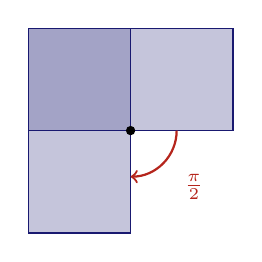
\begin{tikzpicture}[scale=1.3,font=\small]
\draw[MidnightBlue,fill=MidnightBlue!25] (0,0) -- (1.0000,0.0000) -- (1.0000,1.0000) -- (0.0000,1.0000) -- cycle;
\draw[MidnightBlue,fill=MidnightBlue!40] (0,0) -- (0.0000,1.0000) -- (-1.0000,1.0000) -- (-1.0000,0.0000) -- cycle;
\draw[MidnightBlue,fill=MidnightBlue!25] (0,0) -- (-1.0000,0.0000) -- (-1.0000,-1.0000) -- (-0.0000,-1.0000) -- cycle;
\draw[BrickRed,thick,->] (0.45,0) arc (0:-90:0.45);
\node[BrickRed] at (0.62,-0.55) {$\frac\pi2$};
\fill (0,0) circle (1.3pt);
\end{tikzpicture}
